\documentclass{article}
\usepackage{amsfonts}
\usepackage[fleqn]{mathtools}
\usepackage{amssymb}
\usepackage[a4paper, total={6.5in, 9in}]{geometry}
\DeclareMathSizes{10}{10}{9}{7}
\hyphenpenalty=10000

\usepackage{graphicx}
\graphicspath{ {./img/} }
\DeclareGraphicsExtensions{.jpg,.png}

\usepackage{hyperref}

\newcommand{\p}{\partial}
\newcommand{\fpd}[2][]{\frac{\partial #1}{\partial #2}}
\newcommand{\spd}[2][]{\frac{\partial^2 #1}{\partial #2}}
\newcommand{\hsp}[1][5]{\hspace{0.#1 cm}}
\newcommand{\hcm}[1][1]{\hspace{#1 cm}}
\newcommand{\bra}[1][1.2]{\scalebox{#1}{$\boldsymbol{\langle}$}}
\newcommand{\ket}[1][1.2]{\scalebox{#1}{$\boldsymbol{\rangle}$}}
\newcommand{\hh}{\hbar}
\newcommand{\dint}[4][0]{\int_{#1}^{#2} #3 \ d#4}
\newcommand{\lt}{\left}
\newcommand{\rt}{\right}
\newcommand{\lcm}{\text{lcm}}
\newcommand{\imp}{\Rightarrow}
\newcommand{\rimplies}{\Longleftarrow}
\newcommand{\rimp}{\Leftarrow}
\newcommand{\siff}{\Leftrightarrow}
\newcommand{\st}{\ : \ }

\newcommand{\N}{\mathbb{N}}
\newcommand{\Z}{\mathbb{Z}}
\newcommand{\Q}{\mathbb{Q}}
\newcommand{\R}{\mathbb{R}}
\newcommand{\C}{\mathbb{C}}
\newcommand{\G}[1][n]{\mathcal{G}_#1}

\newcommand{\ch}[1]{\text{#1}}
\newcommand{\tdeg}{$^{\circ}$}
\newcommand{\mdeg}{^{\circ}}

\makeatletter
\newcommand*\bigcdot{\mathpalette\bigcdot@{.5}}
\newcommand*\bigcdot@[2]{\mathbin{\vcenter{\hbox{\scalebox{#2}{$\m@th#1\bullet$}}}}}
\makeatother
\newcommand{\inr}{{\mspace{2mu}\bigcdot\mspace{2mu}}}
\newcommand{\otr}{\raisebox{0.1ex}{\scalebox{0.7}{$\boldsymbol{\wedge}$}}}
\newcommand{\x}{{\times}}
\newcommand{\rev}{^\dag}
\newcommand{\nsubg}{\trianglelefteq}

\newcommand{\FLIPINDEX}[1]{{\scalebox{1}[-1]{$\scriptscriptstyle{#1}$}}}
\newcommand{\FLIPARG}[1]{{\scalebox{1}[-1]{$\mkern2mu#1$}}}


\newcommand{\dspt}{\displaystyle} 
\newcommand{\mycomment}[1]{}

\begin{document}
\begin{center}
Nonstandard Analysis - Alain Robert
\end{center}
\begin{flushleft}
\hangindent=1cm 

\textbf{Idealization Axiom:}\\\hcm
$\forall^{sf} F\ \ \exists x\ R(x,F) \iff \exists x\ \forall^{s} y\ R(x,y)$\\[6pt]

\textbf{Standardization Axiom:}\\\hcm
$\dspt \forall P(x)\ \ \exists^s A\subseteq E\ \ \ \forall^sx\ \big(x\in A \iff x\in E \ch{ and } P(x) \big)$\\\hcm($E$ is some parent set)\\[6pt]

\textbf{Transfer Axiom:}\\\hcm
For any standard parameters $A, B, ..., L$ of a \textbf{classical} formula $F$:
$\forall^s x\ F(x, A, B, ..., L) \iff \forall x\ F(x, A, B, ..., L)$\\[4pt]\hcm
letting $F' = \neg F$ gives the equivalent $\exists x\ F'(x, A, B, ..., L) \iff \exists^s x\ F'(x, A, B, ..., L)$\\[4pt]\hcm
By the dual form, all objects uniquely defined by classical formulas are both unique and standard.\\[4pt]\hcm
Note: in general not all properties $P(x)$ are set-forming, but we can always create a standard set $\vphantom{k}^s\{x\in E \st P(x)\}$\\[4pt]\hcm
Example to think about: for $v$ illimited, the interval in $\N$ of $[0,v] \subset \N$ but $\vphantom{k}^s[0,v] = \N$...\\\ \\\ \\\ 


\hypertarget{wellorder}{\textbf{Well-Ordering Principle of the Natural Numbers:}}\\\hsp
\textbf{``Every nonempty subset of $\N$ has a smallest element"}\\\ \\\ 
Induction comes from this well-ordering principle:\\[6pt]\hsp
$P(x)$ is true for $x=0$ and $P(n) \imp P(n+1)$ means $P(x)$ holds for all $x\in \N$.\\[6pt]\hsp\hsp
Convert to a set so we can justify by the well-ordering principle: $T = \{x \in \N \st P(x)\},\ F = \N/A$. Assume the premise and that $F \neq \emptyset$, so $F$ must have a least element $f$. However, since $N=T+F$, $f-1 \in T$ and $P(f-1) \imp P(f)$, a contradiction. So $F$ must be empty.\\[6pt]\hsp
So as long as we can \textit{properly} form the set $T$ (see below), we can apply induction without further thought (see \hyperlink{2.8.4}{exercise 2.8.4}).\\\ 

$P$ being \textbf{set-forming} in $E$ implies (means?): letting $F = \{x \in E \st P(x)\}$\\\hcm\hsp $\forall x \in F\ \ P(x)$ and $\forall x \in E/F\ \ \neg P(x)$\\[6pt] 
\textbf{Set-forming nonexample:} $P(x) = $ ``$x$ is standard", form $\{x \in \N \st P(x)\}$\\\hcm
Suppose $P(x)$ set forming and that this set is finite; then the set of illimited integers has a smallest element $b$ for which $b-1 = n$, where $n$ is standard. However, transfer applies to the formula $b = n+1$, so $b$ must be standard too, a contradiction. Hence the set of standard integers must be infinite. However, every infinite set of integers contains illimited integers by idealization, so $P(x)$ does not hold for some elements in the set, hence $P(x)$ is not set-forming in $\N$.\\[6pt]\hcm Note the converse is not true: given an illimted $n$, $[0,n]$ is nonstandard (invert theorem 2.4.2), but we are still forbidden from collecting all the standard elements here.\\\ 

\hypertarget{non2}{\textbf{nonexample 2:}} From a standard and infinite $E$ and same $P(x)$, form $T = \{x \in E \st P(x)\}$\\\hcm Suppose $P(x)$ set forming and $T$ finite, so $T$ must be standard (theorem 2.4.2). Then, due to sharing exactly the same standard elements, transfer applies and we have $T=E$, a contradiction. So $T$ must be infinite. Since any infinite set contains nonstandard elements (apply idealization to the $\neq$ relation), $T$ contains nonstandard elements, hence $P(x)$ is not set forming in standard infinite sets.\\[6pt]\hcm
This complements theorem 2.4.2:\\\hcm
For infinite standard sets, ``$x$ is standard" must not be set-forming (just proved).\\\hcm
A finite set is standard $\iff$ all elements are standard (2.4.2).\\\ \\\ \\\ 



\textbf{Exercises 1.9} (didn't know how to solve \#3 without axioms from the next chapter???)\\\ 

\hsp 1.9.1: To do this without axioms from chapt 2 requires an inductive argument, which I did type up before, but I deleted it for some reason and am too lazy to type up again because annoying :)\\\ \\\hcm Injective and surjective are classical properties, hence we can form the classical statement\\\hsp\hsp $P(x) = $ ``an injective map of x to itself is surjective".\\\hcm This is true for all standard intervals of $\N$: an injective map from $[0,n-1]$ implies the image must have cardinality $n$. Since the codomain also has size $n$, the map is surjective.\\\hcm Since $P(x)$ is classical, transfer applies and $P(x)$ holds for all intervals $[0,n]\subset \N$, including illimited $n$.\\\ 

\hsp 1.9.2: Let $n$ be illimited and form the infinite set $S = \{1\} \cap \{n,\ n+1,\ n+2,\ ...\}$ Then the property forming $T = \{x \in S \st x \ch{ is standard}\}$ is set forming: 1 is standard, and all elements of $S/T$ are nonstandard (this shows $S$ is nonstandard, see \hyperlink{non2}{nonexample 2}).\\\ \\\hcm
Let $n$ be illimited and form the set $\{1, n\}$. By the same reasoning above, the property ``$x$ is standard" is set-forming here. (also note this set is nonstandard by the inversion of theorem 2.4.2)\\\ 

\hsp 1.9.3: All 3 propositions are false. Counterexample: for every standard integer $n$, $2^n > n$, so transfer applies: for any illimited integer $n$, $n < 2^n$, so $2^n$ is also illimited.\\\

\hangindent=0cm
\textbf{For positive $x$ illimited and $a$ limited, $x-a$ is illimited (and thus also nonstandard).} Suppose the contrary: $x-a = b$, for some $b$ limited. Then $x = a + b$, which by $F'$, would imply $x$ is standard, contradictory to $x$ being illimited. \\\ 

\hangindent=1cm
\textbf{Exercises 2.8}\\\ 

\hsp \hypertarget{2.8.1}{2.8.1:} Suppose we had a standard nonempty set with all nonstandard elements. Then the property ``$x$ is standard" would be set-forming here, and \hyperlink{non2}{nonexample 2} implies this set must be finite, but inversion of theorem 2.4.2 says this set is then nonstandard, a contradiction. So any standard nonempty set must have at least one standard element.\\\ 

\hsp 2.8.2: A standard infinite set must have infinite nonstandard elements, otherwise by listing the nonstandard elements in a set and taking the difference we'd obtain that ``$x$ is standard" is set-forming, a contradiction by \hyperlink{non2}{nonexample 2}. By the same example, any infinite set of all nonstandard elements must be nonstandard, as ``$x$ is standard" is set-forming in this set.\\\ 

\hsp 2.8.3: The projections (two standard functions) uniquely define the sets $E$ and $F$ from $E\times F$, so $E$ and $F$ are both standard.\\\ 

\hsp \hypertarget{2.8.4}{2.8.4:} Continuing \hyperlink{wellorder}{the earlier discussion on induction}, for any (classical or not) property $P$, standardization says we can always form $T = \vphantom{k}^s\{x \in \N \st P(x)\}$. Then $F = \N/T$ is also standard. Should $P(0)$ hold and $\forall^s n\ P(n) \imp P(n+1)$, then $F$ must be empty (see the earlier discussion, it fits right in). So the conclusion that $P(n)$ holds for all standard $ n\in \N$ holds.\\\ 

\hsp 2.8.5: B and C are obviously standard. Take $D = C/A = \{x\in \Q \st 0\leq x < \varepsilon\}$. D must be nonstandard as ``$x$ is standard" is set forming. So supposing $A$ standard immediately leads to contradiction as this would uniquely define $D$ via a standard formula, hence $A$ is nonstandard.\\\ 

\hsp 2.8.6: Form 	























\mycomment{
\hangindent=0cm
Last one is quickest: If the vector field $F$ is conservative, then it comes from some scalar field $s$ like so: $$F =  \nabla s$$
So just take the curl of the vector field. If it is indeed conservative, then the curl will be 0 everywhere, as the curl of any gradient is 0:
$$\nabla \times F = \nabla \times \nabla s = 0$$
As for why the curl of a gradient is 0... this is a very informal explanation, but think of gradient as measuring how the scalar field changes \textit{with space}. I.e. it "adds" a spatial component in to form the vector field $\nabla s$. The curl looks at how it changes against space, rotating from one coordinate to another at a point rather than going anywhere. But the only change in $\nabla s$ is with space. Hence $\nabla \times \nabla s = 0$. If you think about this for a while and it doesn't make sense, just ignore it and remember $\nabla \times \nabla$ is 0 lol\\\ 


In a gist, this is what we want out of a line integral: Given a scalar function over a space and a path in that space, how do we ``add up" (integrate) the scalar function over the whole path?\\\ 
\begin{center}
	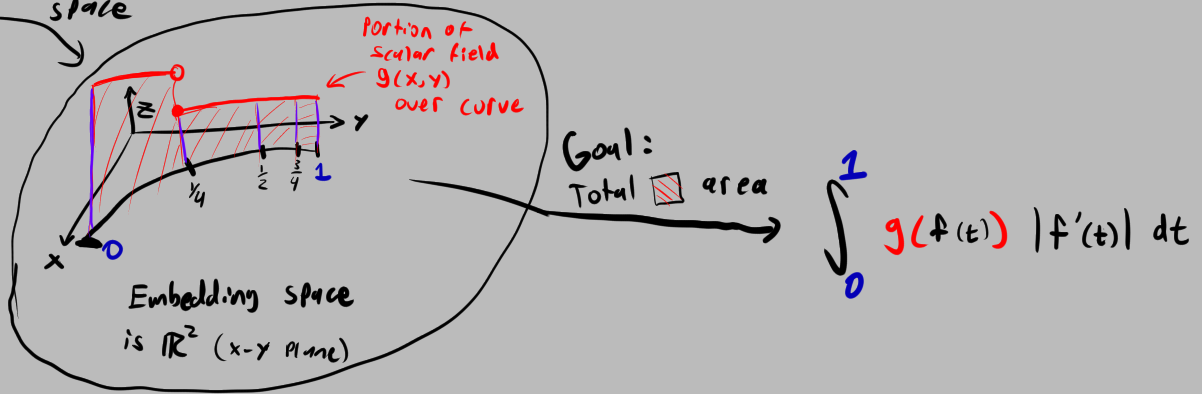
\includegraphics[width=12cm]{int}
\end{center}
In this case, the space is $\R^2$ (x-y plane), and the path the tick-marked curve (black). Plotting our scalar function directly over the path looks like $z = g(x,y)$ (red line). What we're doing when we integrate is figuring out the total red-shaded area.\\\ 

To break it down, first we need to be able to describe our path in a form that makes it convenient to take an integral. Well, we know how to integrate over intervals with definite integrals from 1-D calc. The parameterization gets us a step towards being able to use our old tool:
\begin{center}
	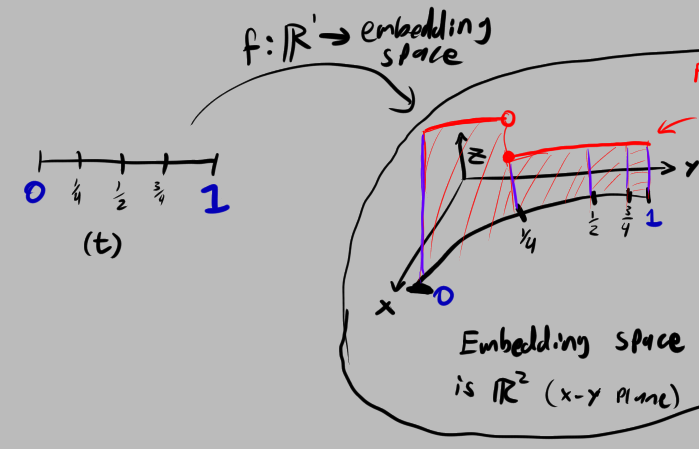
\includegraphics[width=10cm]{line}
\end{center}
What we do is take an interval (say, $[0,1]$) and warp it into the shape of our curve using some function $f$, which takes in a real number and spits out a point on the curve.\\ ``Find a parameterization" means to find a function which takes some line segment and turns it into your desired curve. The details are completely up to you, doesn't matter how you do it as long as it does this task.\\\ 

So in our case, if we take $f(t)$ as our parameterization, by moving $t$ from 0 to 1 we can traverse our desired curve to integrate over, traveling by the output of $f(t)$. Can we just stick $g(f(t)) \ch{d}x$ in our integral, say we integrated the scalar function over the curve and call it a day?\\\ \\
\begin{center}$\dspt \int_0^1 g(f(t))\ \ch{d}t$\\\ \\The Line Integral (do not do this)\\\ \\\end{center}
Look at the diagram of what we want again, the area of the shaded red part:\\\ \\
\hcm[2] 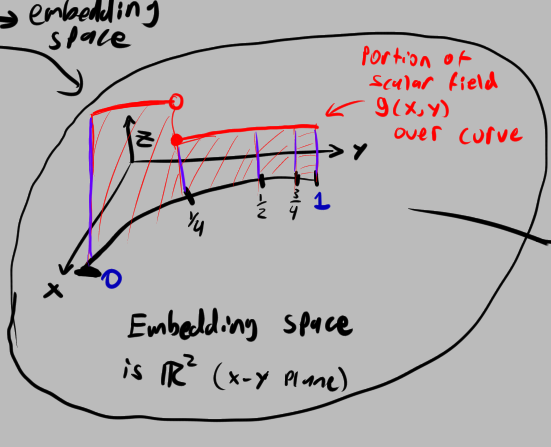
\includegraphics[width=8cm]{form}\\\ \\
We want the section that goes from 0 to $1/4$ to count more than the section from $3/4$ to 1. The integral we wrote earlier weights all these segments equally. It's not what we want!\\\ 

For a more concrete example, consider a line 7 units long in $\R^2$ and parameterized by $f(t) = 3\hat{x} + 7t \hat{y}$:\\\ \\
\hcm[2] 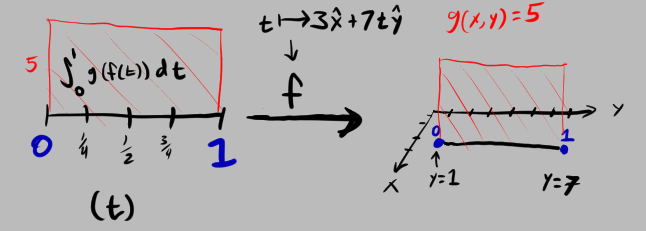
\includegraphics[width=8cm]{sim}\\\ \\
\hcm[1](the $\hat{x}$ and $\hat{y}$ are unit vectors in the $x$ and $y$ directions, respectively)\\\ 

From the picture, we know for the constant function $g(x,y) = 5$, the shaded area should be $7\times 5 = 35$.\\But the integral $\dspt \int_0^1 g(f(t)) \ch{d}t = \int_0^1 5\ \ch{d}t = 5$. We're not accounting for how the parameterization stretches out the line segment $[0,1]$. Currently what we're doing is ``squishing" the portion of $g(x,y)$ over our curve in $\R^2$ into the interval $[0,1]$, and just integrating that instead. We need a way to avoid this ``squish".\\\ 

The fix is simple: If $f$ is our parameterization from interval to curve, then for every tiny interval piece d$t$, $|f'(t)|$d$t$ is the length of the corresponding piece on the curve.\\\ 

Think hard about this. Does it account for a constant stretch of the interval like in our simple example? Now think of a general parameterization as approximated by lots of different constant stretches and squishes of the interval, all strung together to make the curve. This is why it doesn't matter what particular parameterization we choose as long as they all spit out the whole curve. The quirks of each will be adjusted for in the end.\\\ 

Hopefully this will make sense. That's why the line integral looks like this:
\begin{center}$\dspt \int_a^b g(f(t))|f'(t)|\ \ch{d}t$\\\ \\The Line Integral\\(for real, where $a$ and $b$ is the start and end points of the interval your parameterization $f$ takes)\\\ \\	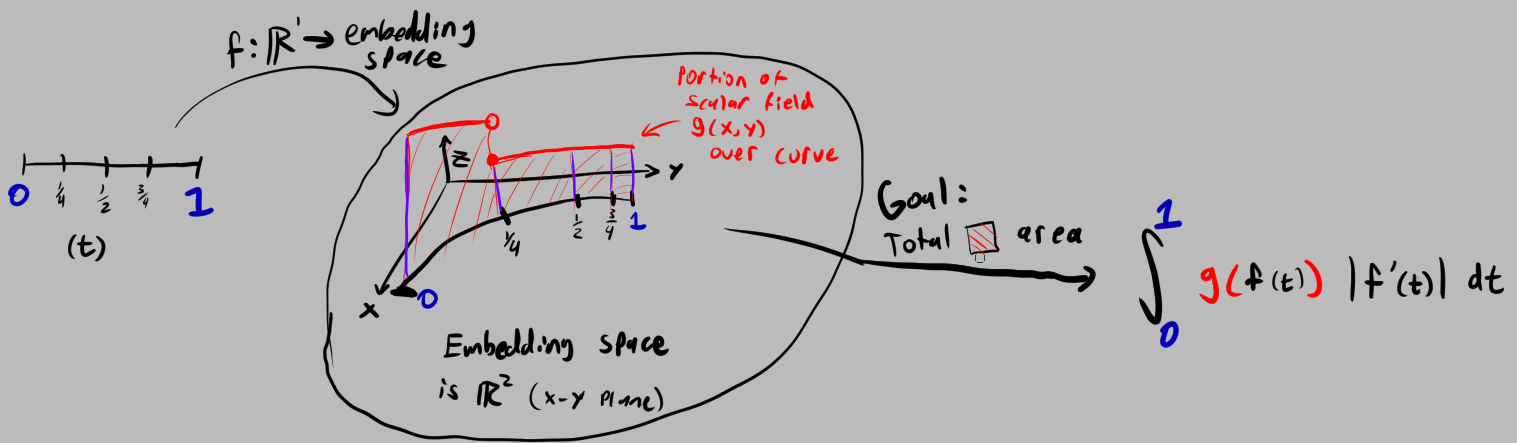
\includegraphics[width=16cm]{whole}\end{center}\ \\\ 

As for the vector line integral, we just want to find the component of the vector field $G$ along the curve parameterized by $f$:\\[6pt]
\hcm $\dspt \int_a^b G(f(t))\inr f'(t)\ \ch{d}t$\\[6pt]
It's very similar to the scalar integral, since we can decompose the tangent vector to the curve into its magnitude and direction:\\[6pt]
\hcm $f'(t) = \hat{f'}(t)|f'(t)|$\\[2pt]
(the hat on $f'$ on the right is to indicate a unit vector in the direction of $f'$)\\[6pt]
So the integrand decomposes into essentially a scalar field over the path, indicating how much of the vector field $G$ is aligned with the path at every point: $g(f(t)) = G(f(t))\inr \hat{f'}(t)$\\\ 

And then we just do our normal scalar line integral:\\\ 

\hcm $\dspt \int_a^b g(f(t))|f'(t)|\ \ch{d}t = \int_a^b G(f(t))\inr \hat{f'}(t)|f'(t)|\ \ch{d}t = \int_a^b G(f(t))\inr f'(t)\ \ch{d}t$\\\ 

So that explains why the vector line integral looks the way it does.
}



\end{flushleft}
\end{document}